\chapter{Hardware design}
Generelt kan det overordnede hardware design beskrives som noget elektronik der sender information ud på nettet, som sendes og analyseres af noget elektronik i den anden ende. Disse vil blive beskrevet herunder som encoder og decoder.  


\section{Encoder}
Encoderen, også omtalt som senderenhed, er den del af systemet der genererer X10 kommandoen og sender den ud på det eksisterende el-net. Et højpasfilter der lader 120 kHz burst passere mens det blokerer for nettets 50 Hz signal, udgør sammen med en zero crossing detector hele hardwaren for encoderen.

\begin{figure}[htbp]
	\centering
	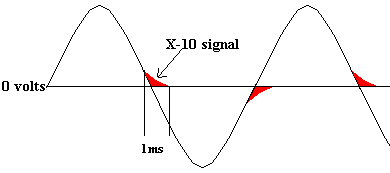
\includegraphics[width=0.50\textwidth]{billeder/HWdesign/X10_BURST}
	\caption{120 kHz burst i zero crossing}
	\label{fig:X10_BURST}
\end{figure}

Ideen med at sende burst ud på nettet i zero crossing kan ses illustreret på figur \ref{fig:X10_BURST}

\begin{figure}[htbp]
	\centering
	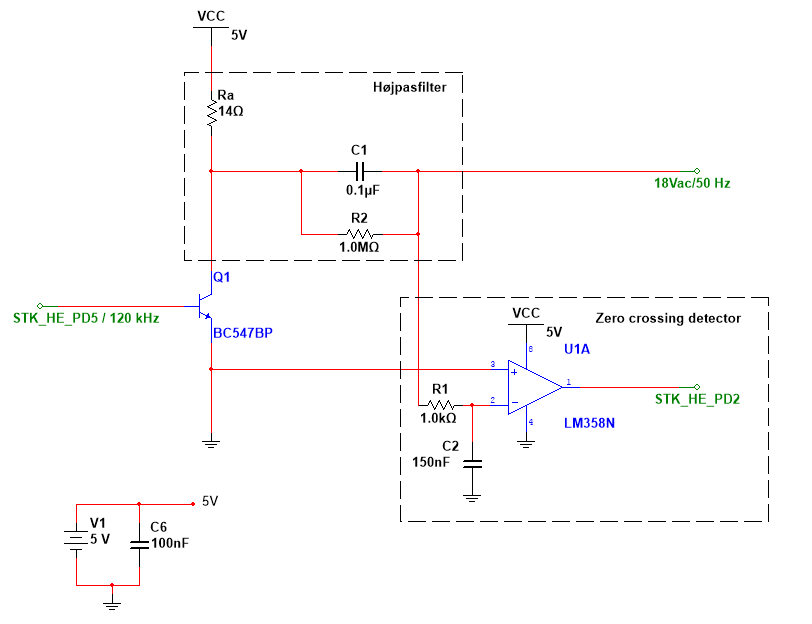
\includegraphics[width=0.70\textwidth]{billeder/HWdesign/Encoder}
	\caption{Samlet Encoder}
	\label{fig:Encoder}
\end{figure}
\newpage

\subsection{Højpasfilter}

\begin{figure}[htb]
  \begin{minipage}{0.45\textwidth}
    \centering
      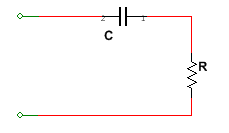
\includegraphics[width=\textwidth]{billeder/HWdesign/HP_UV}
      \caption{Højpasfilter uden værdier}
    \label{fig:HP_UV}
  \end{minipage}
  \hspace{0.1\textwidth}
  \begin{minipage}{0.45\textwidth}
    \centering
      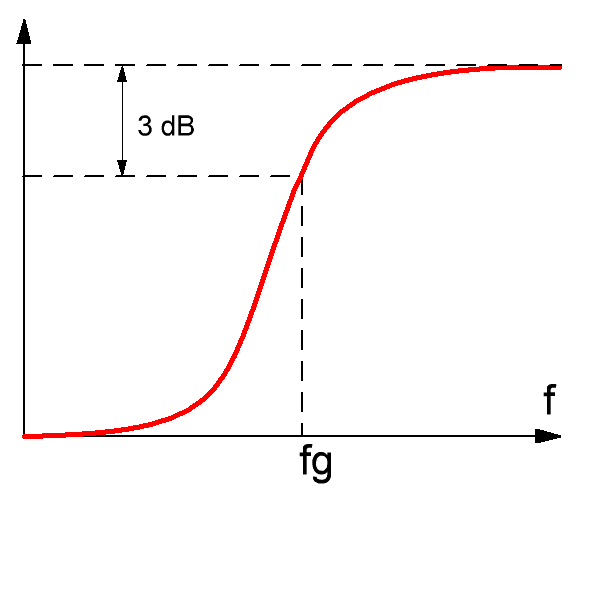
\includegraphics[width=\textwidth]{billeder/HWdesign/HP_KURVE}
      \caption{Kurvekarakteristik for højpasfilter}
    \label{fig:HP_KURVE}
  \end{minipage}
\end{figure}

For at sende X10 kommandoer ud på det eksisterende 50 Hz el-net er det nødvendigt at koble elektroniken direkte herpå og eftersom det elektronik ikke tåler de høje spændinger fra nettet, er det nødvendigt at blokere det signal, men stadig at kunne sende de 120 kHz ud. Dette løses med et højpasfilter.

Den ønskede knækfrekvens skal ligge omkring de 120 kHz for at opnå mindst dæmpning herpå. Ved denne knækfrekvens skulle 50 Hz signalet være ubetydelig lille efter filteret. 

Kondensatoren forudbestemmes for beregningerne til en værdi på 0,1 nF.

\begin{align}
R_1 = \frac{1}{2 \cdot \pi \cdot f_c \cdot C } = \frac{1}{2 \cdot \pi \cdot 120000 \cdot 0,1 \cdot 10^{-6}} = 13,26 \Omega
\rightarrow R_1 > 13,26 \Omega
\end{align}
$R_1$ vælges da til 14 $\Omega$

Med den beregnede modstands værdi er det endelige schematic færdigt som det ses på figur \ref{fig:HP_MV}

\begin{figure}[htbp]
	\centering
	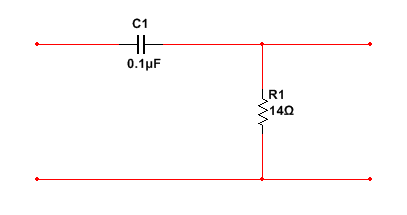
\includegraphics[width=0.50\textwidth]{billeder/HWdesign/HP_MV.png}
	\caption{Højpasfilter med værdier}
	\label{fig:HP_MV}
\end{figure}

\newpage
  
\subsection{Zero Crossing Detector}
\begin{figure}[htb]
  \begin{minipage}{0.45\textwidth}
    \centering
      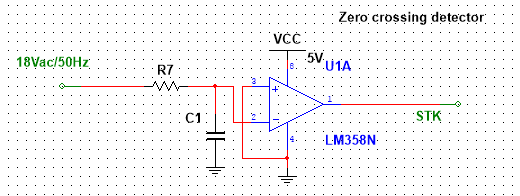
\includegraphics[width=\textwidth]{billeder/HWdesign/ZC_UV}
      \caption{Zero crossing detector uden værdier}
    \label{fig:ZC_UV}
  \end{minipage}
  \hspace{0.1\textwidth}
  \begin{minipage}{0.45\textwidth}
    \centering
      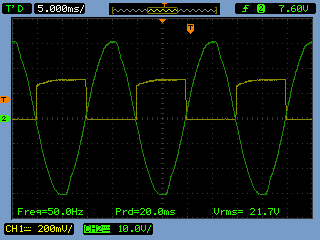
\includegraphics[width=\textwidth]{billeder/HWTest/Encoder/Encoder_zerocross}
      \caption{Scope billede af Zero crossing detector, CH1(indgangssignal), CH2(Udgangssignal)}
    \label{fig:Encoder_Zerocross}
  \end{minipage}
\end{figure}

Zero crossing detectoren har til opgave at detektere nulgennemgang, det er et krav for at X10 protokollen kan virke. Der er placeret en Zero crossing detector både på Encoderen og Decoderen, da begge disse består af et STK-kit der kræver information om nulgennemgang. Opbygning kan ses på overstående figur \ref{fig:ZC_UV}, der er anvendt en operationsforstærker af typen LM358N\footnote{Se bilag ??? for datablad}, som toggler udgangssignalet ved hver nulgennemgang se figur \ref{fig:Encoder_Zerocross}. Operationsforstærkerens positive ben er koblet til stel for at lave et triggerniveau til 0 V.

Modstanden $R_7$ sidder der bl.a. for at beskytte Zero crossing detectoren mod 18 VAC nettet, men sammen med kondensatoren udgør den også et lavpasfilter. Under implementeringen kunne det konstateres at der kom støj ind på Zero crossing detectoren, og dette problem løste lavpasfilteret. 

Der ønskes at dæmpe 120 kHz signalet, derfor designes lavpasfilteret ud fra en knækfrekvens på 1,0 kHz. 

\begin{align}
R = \frac{1}{2 \cdot \pi \cdot f_c \cdot C } 
\end{align}

Der vælges en kondensator med en værdi på 150 nF. Med denne værdig kan modstanden i lavpasfilteret beregnes. 

Lavpasfilterets modstand:
\begin{align}
R_7 = \frac{1}{2 \cdot \pi \cdot \ 1000 \cdot 150 \cdot 10^{-9}} = 1061 \Omega
\end{align}
$R_7$ vælges da til 1,0 k$\Omega$

Med alle de beregnede komponentværdier kan det endelige schematic designes. Det endelige design er vist på figur \ref{fig:ZC_MV} 

\begin{figure}[htbp]
	\centering
	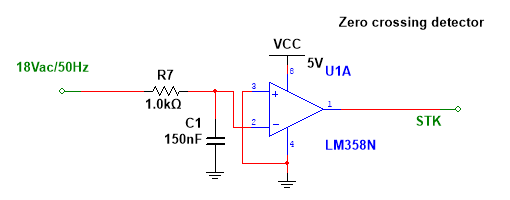
\includegraphics[width=0.70\textwidth]{billeder/HWdesign/ZC_MV}
	\caption{Zero crossing med værdier}
	\label{fig:ZC_MV}
\end{figure}

\newpage

\section{Decoder}
Decoderen, som er den del i systemet der omdanner burst fra encoderen til X10 kommando, er opbygget af et båndpasfilter, zero crossing detector og en envelope detector. I starten af kredsløbet sidder båndpasfilteret, og dette blokerer for 50 Hz nettet og forstærker 120 kHz signalet der kommer fra encoderen. Herefter ledes signalet gennem envelope detector som omdanner burstet til et TTL signal.

\begin{figure}[htbp]
	\centering
	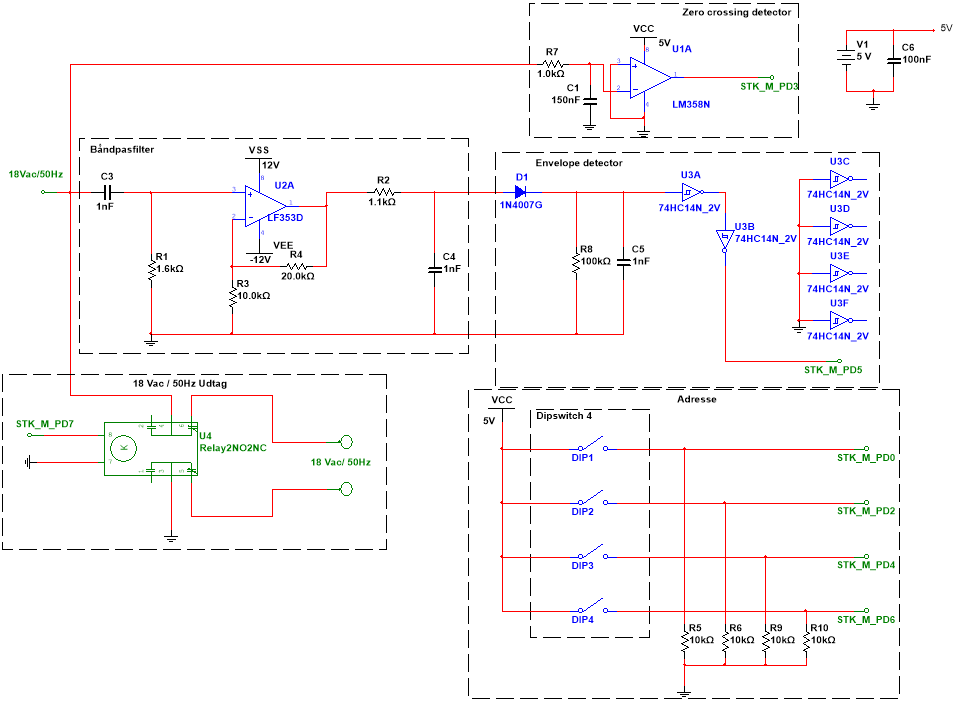
\includegraphics[width=0.70\textwidth]{billeder/HWdesign/Decoder}
	\caption{Samlet Decoder}
	\label{fig:Decoder}
\end{figure}


\newpage

\subsection{Båndpasfilter}

\begin{figure}[htb]
  \begin{minipage}{0.45\textwidth}
    \centering
      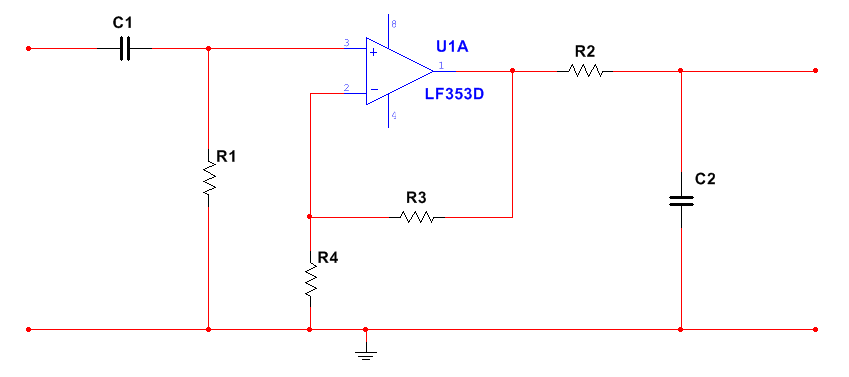
\includegraphics[width=\textwidth]{billeder/HWdesign/BAANDPAS_UV}
      \caption{Båndpasfilter uden værdier}
    \label{fig:BAANDPAS_UV}
  \end{minipage}
  \hspace{0.1\textwidth}
  \begin{minipage}{0.45\textwidth}
    \centering
      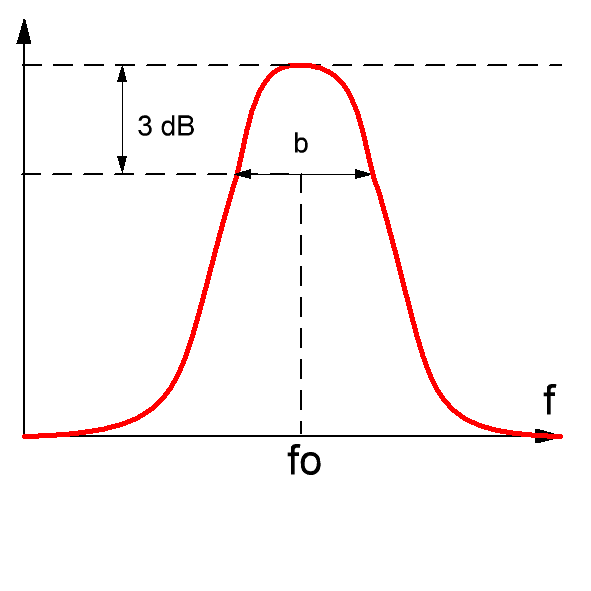
\includegraphics[width=\textwidth]{billeder/HWdesign/BAANDPAS_KURVE}
      \caption{Kurvekarakteristik for båndpasfilter}
    \label{fig:BAANDPAS_KURVE}
  \end{minipage}
\end{figure}

Båndpasfilteret har til opgave at filtrere alle signaler med frekvenser over og under 120 kHZ fra samtidig med at det forstærker signalet i båndpasset. Forstærkningen opnås ved at koble en ikke inverterende OpAmp med modstande, hvis størrelse afhænger af den ønskede forstærkning, mellem et højpasfilter og lavpasfilter som illustreret på figur \ref{fig:BAANDPAS_UV}. Kurvekarakteristikken er illustreret på figur \ref{fig:BAANDPAS_KURVE}.

Da vi ønsker at forstærke 120 kHz signalet, designes højpasfilteret således at knækfrekvensen udregnes til 110 kHz, og for lavpasfilteret beregnes en knækfrekvens på 130 kHz. 

\begin{align}
R = \frac{1}{2 \cdot \pi \cdot f_c \cdot C } 
\end{align}

Fælles for begge filtre vælges en kondensator med en værdi på 1,0 nF. Med denne værdig kan de to modstande i henholdsvis lavpas- og højpasfilteret beregnes.

Højpasfilterets modstand:
\begin{align}
R_1 = \frac{1}{2 \cdot \pi \cdot 110000 \cdot 1,0 \cdot 10^{-9}} = 1447 \Omega
\rightarrow R_1 > 1447 \Omega
\end{align}
$R_1$ vælges da til 1,6 k$\Omega$


Lavpasfilterets modstand:
\begin{align}
R_2 = \frac{1}{2 \cdot \pi \cdot \ 130000 \cdot 1,0 \cdot 10^{-9}} = 1225 \Omega
\rightarrow R_2 < 1224 \Omega
\end{align}
$R_2$ vælges da til 1,1 k$\Omega$

Da det ikke kan undgås at 120 kHz signalet bliver dæmpet både gennem højpasfilteret og lavpasfilteret er det nødvendigt at forstærke signalet ved hjælp af en LF353 OpAmp.
Ligningen for udregning af udgangsspændingen er som følgende:
\begin{align}
V_{out} = (1 + \frac{R_3}{R_4}) \cdot V_{in}
\end{align} 

Ved at vælge $R_4$ til 10 k$\Omega$ kan forstærkningen nemt reguleres med $R_3$.
Ved målinger på indgangssignalet før operationsforstærkeren kan vi fastslå indgangsamplituden til at være 8,0 V. Da udgangssignalet ledes gennem en diode der fjerner de negative halvperioder vil amplituden blive halveret gennem denne. Samtidig er der dæmpning i lavpasfilteret og der vil derfor være brug for en mere end en fordobling i forstærkeren. 

\begin{align}
R_4 = (\beta - 1) \cdot R_3 = (3 - 1) \cdot 10000 = 20000 \Omega
\end{align} 
$R_4$ er valgt til 20000 $\Omega$ så signalet derved bliver forstærket 3 gange.

Der er som nævnt valgt en LF353 OpAmp. Denne er valgt ud fra at den har en bred båndbredte, en hurtig sætte tid og lav støj på indgangene. 

Med alle de beregnede komponentværdier kan det endelige schematic designes. Det endelige design er vist på figur \ref{fig:BAANDPAS_MV} 

\begin{figure}[htbp]
	\centering
	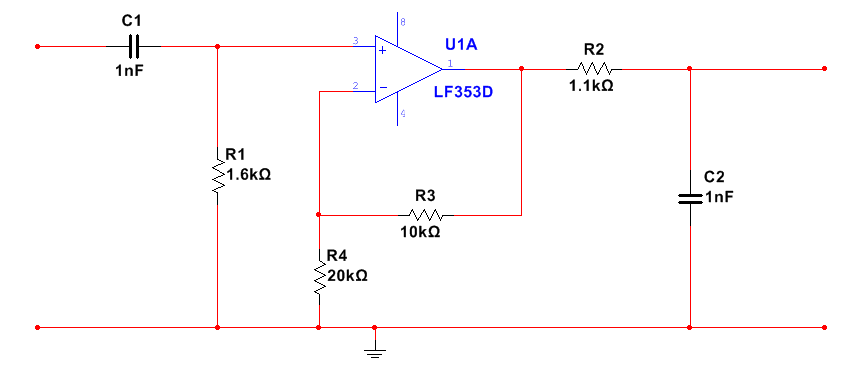
\includegraphics[width=0.70\textwidth]{billeder/HWdesign/BAANDPAS_MV.png}
	\caption{Båndpas med værdier}
	\label{fig:BAANDPAS_MV}
\end{figure}
 

\newpage

\subsection{Envelope Detector}

\begin{figure}[htbp]
	\centering
	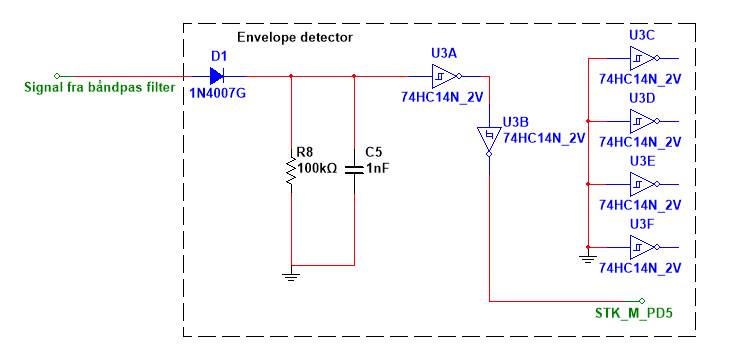
\includegraphics[width=0.70\textwidth]{billeder/HWdesign/ED_MV.png}
	\caption{Envelope detector}
	\label{fig:ED_MV}
\end{figure}

Envelope detectorens opgave er at udglatte burstsignalet fra båndpasfilteret og lave det om til et TTL (0-5V) signal som STK-kitten kan aflæse.

Den er opbygget af en diode, et RC-led og en schmitt trigger. Dioden har til opgave at sortere alle de negative halvperioder fra og kun sende de positive halvperioder til RC-leddet. Kondensatoren vil derfor kun opfange de positive halvperioder, og undgå at belaste det foranliggende kredsløb ved at aflade de negative halvperioder. Kondensatoren er med til at udglatte signalet da den ikke kan nå at aflades på en periode.

Modstanden $R_8$ er en afladningsmodstand, og den bestemmer hvor hurtigt kredsløbet skal aflades, jo højere modstand jo langsommere går det med at aflade. Vi har beregnet modstanden på følgende måde.

Tidskonstanten beregnes til.
\begin{align}
\tau = 120000^{-1} Hz = 8,33 \cdot 10^{-6} s
\end{align}


Kondensatoren bestemmes til at være 1 nF, og modstand $R_8$ kan derfor beregnes ud fra denne formel.
\begin{align}
\tau = R \cdot C 
\end{align}
\begin{align}
R = \frac{\tau}{C} = \frac{8,33 \cdot 10^{-6}}{1 \cdot 10^{-9}} = 83 k\Omega
\end{align}

Modstanden $R_8$ er rundet op til $100 k\Omega$, dette gør at vi er helt sikre på at kondensatoren ikke aflader for hurtigt. 

Der er anvendt en schmitt trigger til at lave signalet om til et firkantet signal som STK-kitten kan aflæses. Grunden til at der er brugt 2 er fordi de er inverterende. 

\newpage
\subsection{Dipswitch}
For at en X10-kommando bliver udført af det korrekte udtag medsendes en adresse på fire bit.
Til at simulere adresseringen for et udtag, er der lavet fire dipswitches der er forsynet med 5 V og forbundet til STK-500 modtageren, som det er illustreret på figur \ref{fig:DIPSWITCH}.

En åben kontakt vil give 0 og en lukket kontakt vil resultere i 1

\begin{figure}[htbp]
	\centering
	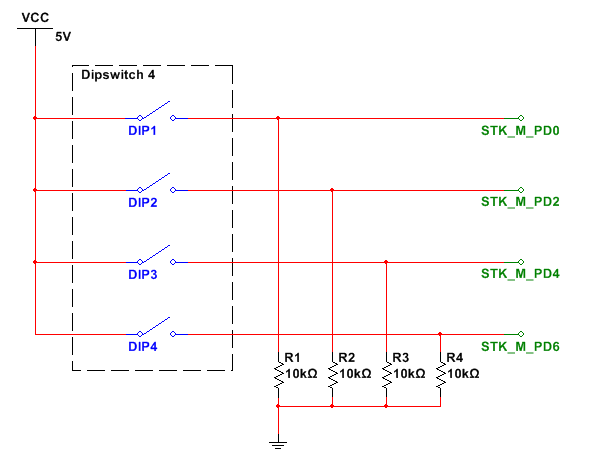
\includegraphics[width=0.70\textwidth]{billeder/HWdesign/DIPSWITCH}
	\caption{Dipswitch for adressering af udtag}
	\label{fig:DIPSWITCH}
\end{figure}

\newpage
\subsection{Komponentliste}

De efterfølgende tabeller viser en oversigt over hvilke komponenter der er anvendt, den beskriver navn, type og størrelse på hver enkelt komponent\footnote{Datablade for komponenterne kan findes i mappen "Datablade" på CD'en•}. 


\begin{table}[htbp] \centering
\caption{Komponentliste over Encoder}
\begin{small}
    \begin{tabular}{|p{2cm}|p{4cm}|p{2cm}|}
    \hline
    \textbf{Navn}    & \textbf{Type}                 & \textbf{Størrelse} \\ \hline
    BC547BP    & Transistor           & ~         \\ \hline
    $R_a$      & Modstand             & 14 $\Omega$    \\ \hline
    $R_2$      & Modstand             & 1 M$\Omega$    \\ \hline
    $R_1$      & Modstand             & 1 k$\Omega$    \\ \hline
    $C_1$      & Kondensator          & 0.1 uF    \\ \hline
    $C_2$      & Kondensator          & 150 nF    \\ \hline
    $C_6$      & Kondensator           & 100 nF    \\ \hline
    LM358N     & Operationsforstærker & ~         \\ \hline
    \end{tabular}
   \end{small}
\label{table:Komponentliste encoder}
\end{table}

\begin{table}[htbp] \centering
\caption{Komponentliste over Decoder}
\begin{small}
    \begin{tabular}{|p{2cm}|p{4cm}|p{2cm}|}
    \hline
    \textbf{Navn}    & \textbf{Type}                 & \textbf{Størrelse} \\ \hline
   
    $R_1$      & Modstand             & 1.6 k$\Omega$    \\ \hline
    $R_2$      & Modstand             & 1.1 k$\Omega$    \\ \hline
    $R_3$      & Modstand             & 10 k$\Omega$    \\ \hline
    $R_4$      & Modstand             & 20 k$\Omega$    \\ \hline
    $R_5$      & Modstand             & 10 k$\Omega$    \\ \hline
    $R_6$      & Modstand             & 10 k$\Omega$    \\ \hline
    $R_7$      & Modstand             & 1 k$\Omega$    \\ \hline
    $R_8$      & Modstand             & 100 k$\Omega$    \\ \hline
    $R_9$      & Modstand             & 10 k$\Omega$    \\ \hline
    $R_{10}$     & Modstand             & 10 k$\Omega$    \\ \hline
    $C_1$      & Kondensator          & 150 uF    \\ \hline
    $C_3$      & Kondensator          & 1 nF    \\ \hline
    $C_4$      & Kondensator          & 1 nF    \\ \hline
    $C_5$      & Kondensator          & 1 nF    \\ \hline
    $C_6$      & Kondensator          & 100 nF    \\ \hline
    LM358N     & Operationsforstærker & ~         \\ \hline
    LF353D     & Operationsforstærker & ~         \\ \hline
    2NO2NC     & Relæ				  & ~         \\ \hline
    74HC14N    & Schmitt trigger	  & ~         \\ \hline
    DIP1       & Kontakt	          & ~         \\ \hline
    DIP2       & Kontakt	          & ~         \\ \hline
    DIP3       & Kontakt	          & ~         \\ \hline
    DIP4       & Kontakt	          & ~         \\ \hline
   
    \end{tabular}
   \end{small}
\label{table:Komponentliste Decoder}
\end{table}
\newpage

\section{DE2-kodelås}

DE2 Boardet bliver brugt som kodelås til CSS Hovedenheden. DE2 Boardet er programmeret i E2DSD Exercise 7\footnote{Se code\_lock.vhd i bilag} som en Statemachine. Der er dog blevet ændret i koden fra øvelsen, da der kun er brug for et enkelt bit til CSS Hovedenheden og ikke en konstant høj. 

\begin{figure}[H]
	\centering
	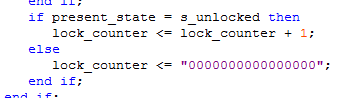
\includegraphics[width=0.70\textwidth]{billeder/HWdesign/code_lock_counter}
	\caption{Lock Counter}
	\label{code:code_lock}
\end{figure}

Figur \ref{code:code_lock} viser en unsigned ved navn lock\_counter, som ligger i state\_reg processen. Den tæller op, når programmet befinder sig i s\_unlocked staten.

\begin{figure}[H]
	\centering
	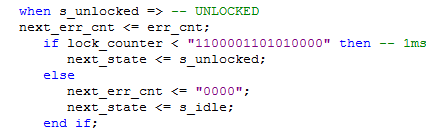
\includegraphics[width=0.70\textwidth]{billeder/HWdesign/code_lock_s_unlocked_state}
	\caption{s\_unlocked}
	\label{code:s_unlocked}
\end{figure}

Figur \ref{code:s_unlocked} viser koden, der fortæller, hvor længe man skal befinde sig i s\_unlocked staten, som sætter LOCK outputtet høj. I dette tilfælde er der valgt 1 ms. Efter 1 ms vil programmet nulstille error-counteren og gå til s\_idle state - klar til nyt input.

Outputtet er sat til GPIO1 JP2 D9 (PIN\_M25), vist i Figur \ref{code:code_lock_pinout}.

\begin{figure}[H]
	\centering
	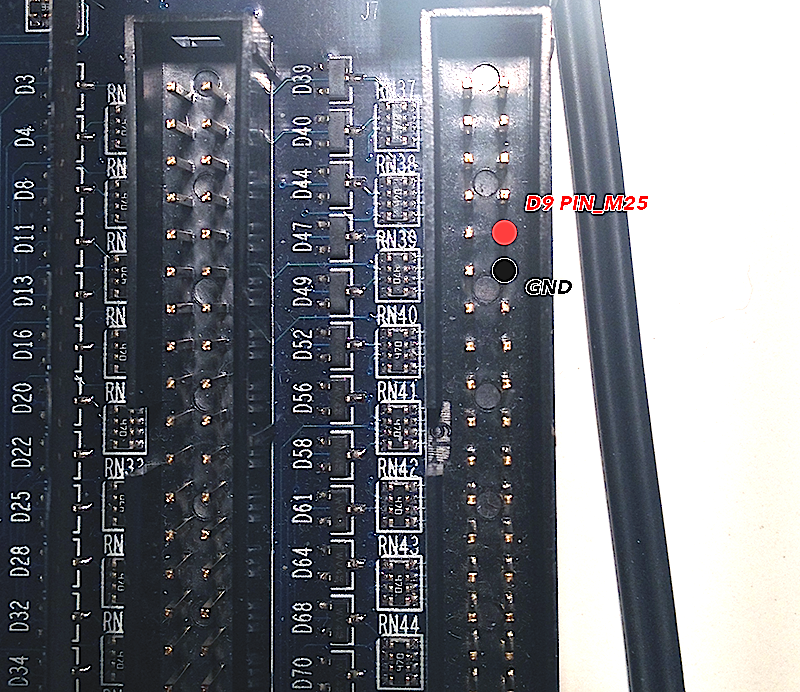
\includegraphics[width=0.40\textwidth]{billeder/HWdesign/code_lock_pinout}
	\caption{DE2-kodelås pinout}
	\label{code:code_lock_pinout}
\end{figure}
\newpage
